\subsection{Normalizing Flows}
\label{subsec:nfs}

\def\valreg{rev_deta}
\def\vallabel{reversed $\Delta \eta_{HH}$}

A normalizing flow is a generative model that transforms a known base density into a desired target density by a sequence of invertible transformations, here denoted $f_i$ \cite{1505.05770}.
By drawing samples from the base distribution and passing these samples through the forward mode of the flow, we obtain samples from the target distribution, which we will use to construct a background prediction for the $m_{HH}$ shape.
The inverse mode of the flow $f^{-1}$ lets us sample from the base distribution then evaluate chain rule of probability. 

\begin{equation}
p_y (y) = p_z(z) \left| \frac{dz}{dy} \right| = p_z (f^{-1}(y)) \left| \frac{df^{-1}}{dy} \right|
\end{equation}
where $p_z(z)$ is the known base density (i.e, a Gaussian), and y is the features we want to model. 

The inverse mode of the flow is how the model is trained by maximum likelihood by taking the loss as the negative log-likelihood of the training data.
Since $y \in \mathbb{R}^d$ is a multi-dimensional variable, these transformations need to be constructed to keep both the Jacobian and the invertibility of the $f_i$s tractable.
To this end, we use a the flow transformation that is a \emph{coupling transform} that transforms groups of variables together to that the $f_i$ matrix stays lower triangular and the Jacobian computation stays $\mathcal{O}(d^2)$.
\Fig{\ref{fig:flow-steps-\valreg}} shows how flow proceeds in 10 steps to gradually transform the base Gaussian density into the Higgs candidate variables in the \vallabel SR.

\begin{figure}[hbt]
    \centering
    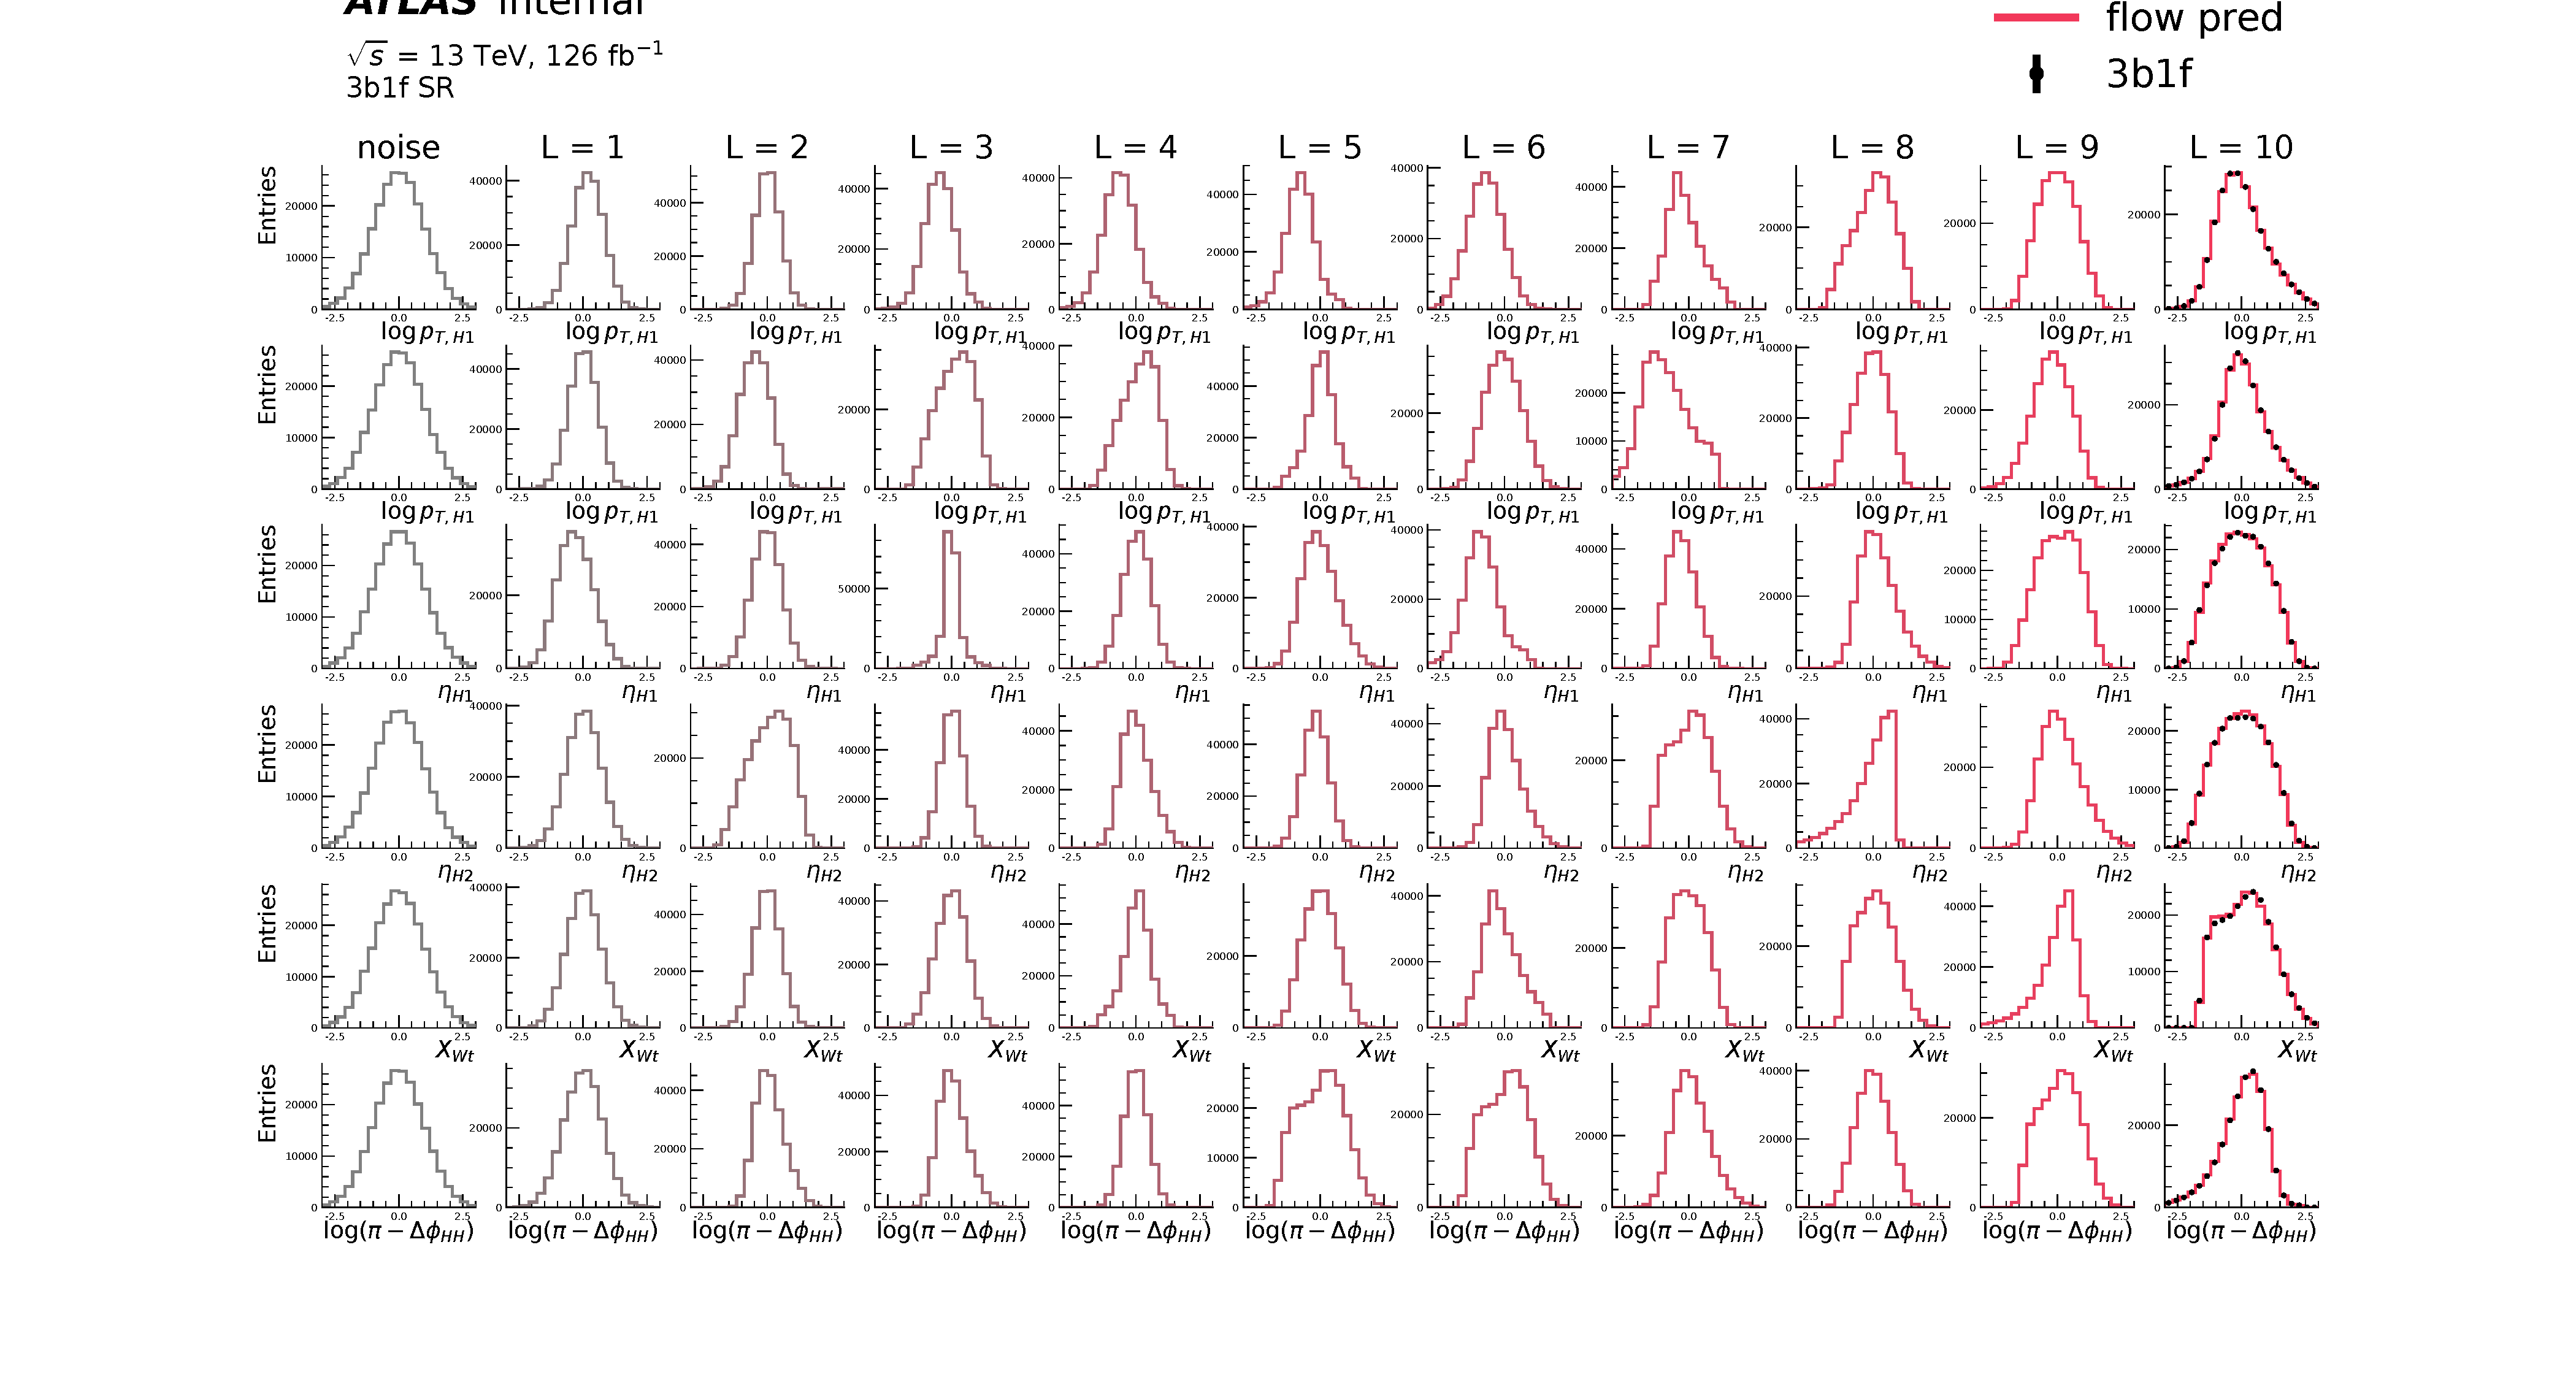
\includegraphics[width=0.92\textwidth]{figures/flows/\valreg/step-by-step-seed0.pdf} 
    \caption{Demonstration of how the flow transforms unstructured noise into a structured prediction in the \vallabel validation region.
    		 These samples are conditioned on the SR $(m_{H1}, m_{H2}, \text{yr} )$ data from the 2016, 2017 and 2018 datasets.
    		 The grey histograms in the left column are samples from a 6d Gaussian.
		 Each column to the right shows the transformation from one layer of the flow (i.e, a single invertible transformation), with the right-most column showing the prediction of the final flow. 
		 This is a single flow training, with the distributions are shown before applying the $X_{Wt}$.
    		 Variables have been scaled to zero mean and unit variance. }  
	 \label{fig:flow-steps-\valreg}
\end{figure}


\FloatBarrier
\clearpage
\subsubsection{Neural Spline Flows}

For recent reviews of various implementations for flow architectures, see reviews \cite{1910.13233, 1912.02762}. In this work, we show a background model for a rational quadratic neural spline flow (RQ-NSF) \cite{1906.04032} which is a universal density approximator in a finite domain if sufficiently many knots for the spline are chosen.

We use the publicly produced repo \cite{https://github.com/bayesiains/nflows} accompanying \cite{1906.04032}, so here briefly summarize the details of the RQ-NSF using the notation from \cite{1906.04032}.

To preserve the tractability of the Jacobain, the modeling vector $y$ is split into two sets of variables $y = [y_{1:m}, y_{m:d}]$, and the variables $y_{m:d}$ are the variables that get transformed while the $y_{1:d}$ are used for the conditioning.

The only constraint needed to ensure the invertibility of $f_i$ is that the $f_i$ are monotonic functions, and here it is chosen to be an increasing function parametrized by a spline with $K$ bins between [B, B] as shown in \Fig{\ref{fig:nsf-graphic}}.

There are $K$ bins giving the internal knots of the transformation, and each "bin" of the domain is a rational quadratic transformation given by:

$$f_{jk}(x_i) = \frac{a_{ijk} x_i^2 + b_{ijk} x_i + c_{ijk} } { d_{ijk} x_i^2 + e_{ijk} x_i + f_{ijk}} $$

where $i$ be the dimension of the transforming variable, and $j$ be the corresponding flow layer.
This transformation can be parametrized by predicting the $2K$ widths and heights of the bins and the $K-1$ derivatives at the internal knots 

This would mean to predict the step of a single transforming variable, we we would need to predict these $6K$ constants: $a_{ijk},b_{ijk},c_{ijk},d_{ijk},e_{ijk},f_{ijk}$.

\begin{minipage}{0.5\textwidth}

 But applying the additional constraints:

\begin{itemize}
	\item Boundary conditions: \textcolor{blue}{$(x_0, y_0) = (-B,-B)$} and \textcolor{yellow}{$(x_K,y_K) = (B,B)$}
	\item Continuity at the internal knots: \textcolor{red}{2(K-1) constraints}
	\item Continuous derivatives at the knots: \textcolor{green}{K-1 constraints}
\end{itemize}

reduces the number of constants to 6K - [ \textcolor{red}{2(K-1)} + \textcolor{green}{2K+1} + \textcolor{blue}{2} + \textcolor{yellow}{2}] = 3K - 1 NN outputs.

\end{minipage}
\hspace{0.05\textwidth}
\begin{minipage}{0.4\textwidth}
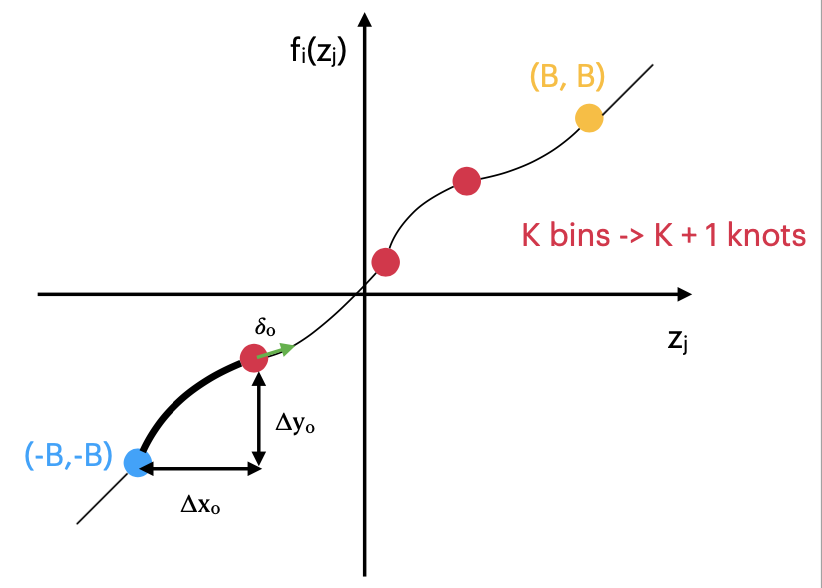
\includegraphics[trim={0 0 1cm 0},width=\textwidth]{figures/flows/flow-architectures/nsf-graphic}
\captionof{figure}{Parmetrization for a RQ-NSF.}
\label{fig:nsf-graphic}
\end{minipage}

So a NN is used to predict an unconstrained $\theta_i \in \mathbb{R}^{3K - 1}$, and then the $\theta_i$ vector is partitioned into three pieces $[\theta_i^w, \theta_i^h, \theta_i^d]$. Since the spline characterizes a transformation from a domain $(-B,B)$ into a range $(-B,B)$, the $\theta_i^w$ and $\theta_i^h$ vectors are each passed through a softmax function (with a range (0,1)) and then multiplied by 2B to give the widths and heights of the shifts between the knot locations.
Since the monoticity of the $f_j$ is crucial for its invertibility, the $\theta_i^d$ are passed through a softplus function to ensure the derivative stays positive as well.
Outside of the range [-B,B] an identify transform is used.

Then instead of taking two sets of variables, this architecture also uses a generalized permutation 

\begin{equation}
	W = P L U,
\end{equation}

where $P$ is the permutation matrix, $L$ is a lower triangular matrix, and $U$ is an upper triangular matrix. % P to allow for random permutations
This is allows additional mixing between the input variables, but the Jacobian stays tractable because $det(W)$ only takes $\mathcal{O}(d)$ time to compute. 
Inverting this step involves solving two triangular systems, which is a $\mathcal{O}(d^2)$ operation. %, the same order as inverting the spline flow operations. (or at least - I think this is what I meant).

Finally, a batch norm layer is used between each of the flow steps to keep the modeling variables in the range where the spline has its expressive power.

\subsubsection{Implementation details}

In practice, we found that it was easier to use the flow model the of the Higgs Candidate 3-momenta instead of modeling the high level $m_{HH}$ and $\Delta \eta_{HH}$ directly. 

We optimized the hyperparameters for this problem by looking at the modeling in the 2b SR.
The architecture we'r using a model is a neural spline flow with 10 layers. The res-net blocks that pre
\begin{itemize}
	\item L=10 
	\item H = 32
	\item \# blocks = 1
	\item K = 4
	\item dropout fraction 0.1
	\item using batch norm
\end{itemize}

We trained with the adam optimizer with a learning rate of $10^{-3}$, and using L2 regularization with $\beta = 1e-6$.
.
Also, to avoid overfitting \ldots

\begin{figure}[hbt]
    \centering
    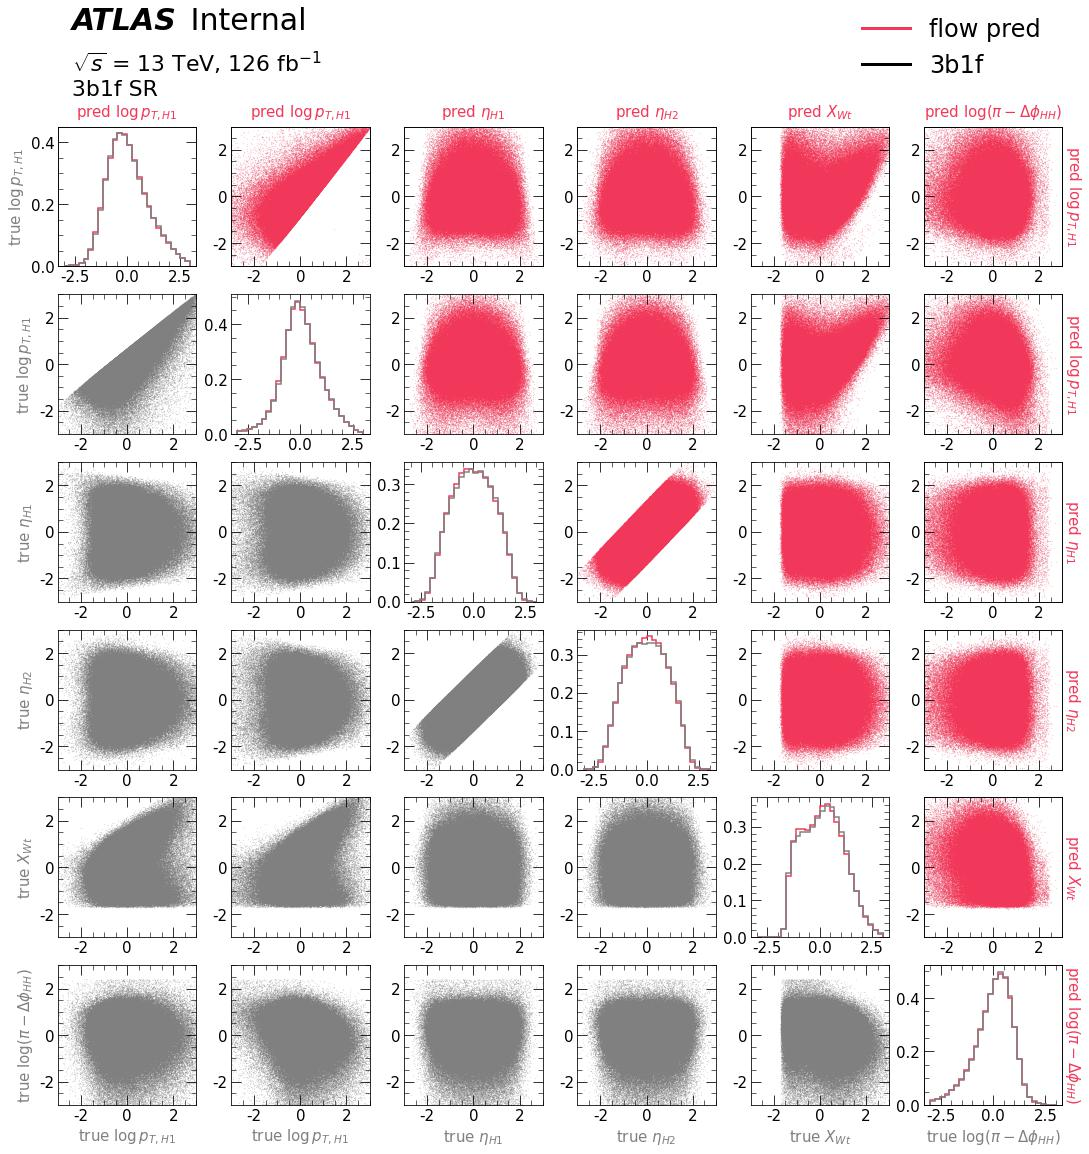
\includegraphics[width=\textwidth]{figures//flows/\valreg/correlation-seed0.jpg} 
    \caption{The correlation between the modeling variables for the SR data (grey) and the flow prediction (pink) in the \vallabel validation region.
    The marginal plots along the diagonal are normalized to unity.
    These samples are conditioned on the SR $(m_{H1}, m_{H2}, \text{yr} )$ data from the 2016, 2017 and 2018 datasets.
    This is a single flow training, with the distributions are shown before applying the $X_{Wt}$.
    Variables have been scaled to zero mean and unit variance.}
    \label{fig:2d-correlation-\valreg}
\end{figure}

Finally, the $X_{Wt}$ cut induces \emph{structure} in the massplane due too the vetoing of HC compatible with the W-mass. So we train our full model before applying the \Xwt cut, but include the \Xwt variable as a modeling variable for the flow so that after the background estimate is trained we can still cut on \Xwt > 1.5 to get the final prediction of the discriminant distribution. 


\begin{figure}[hbt]
    \centering
    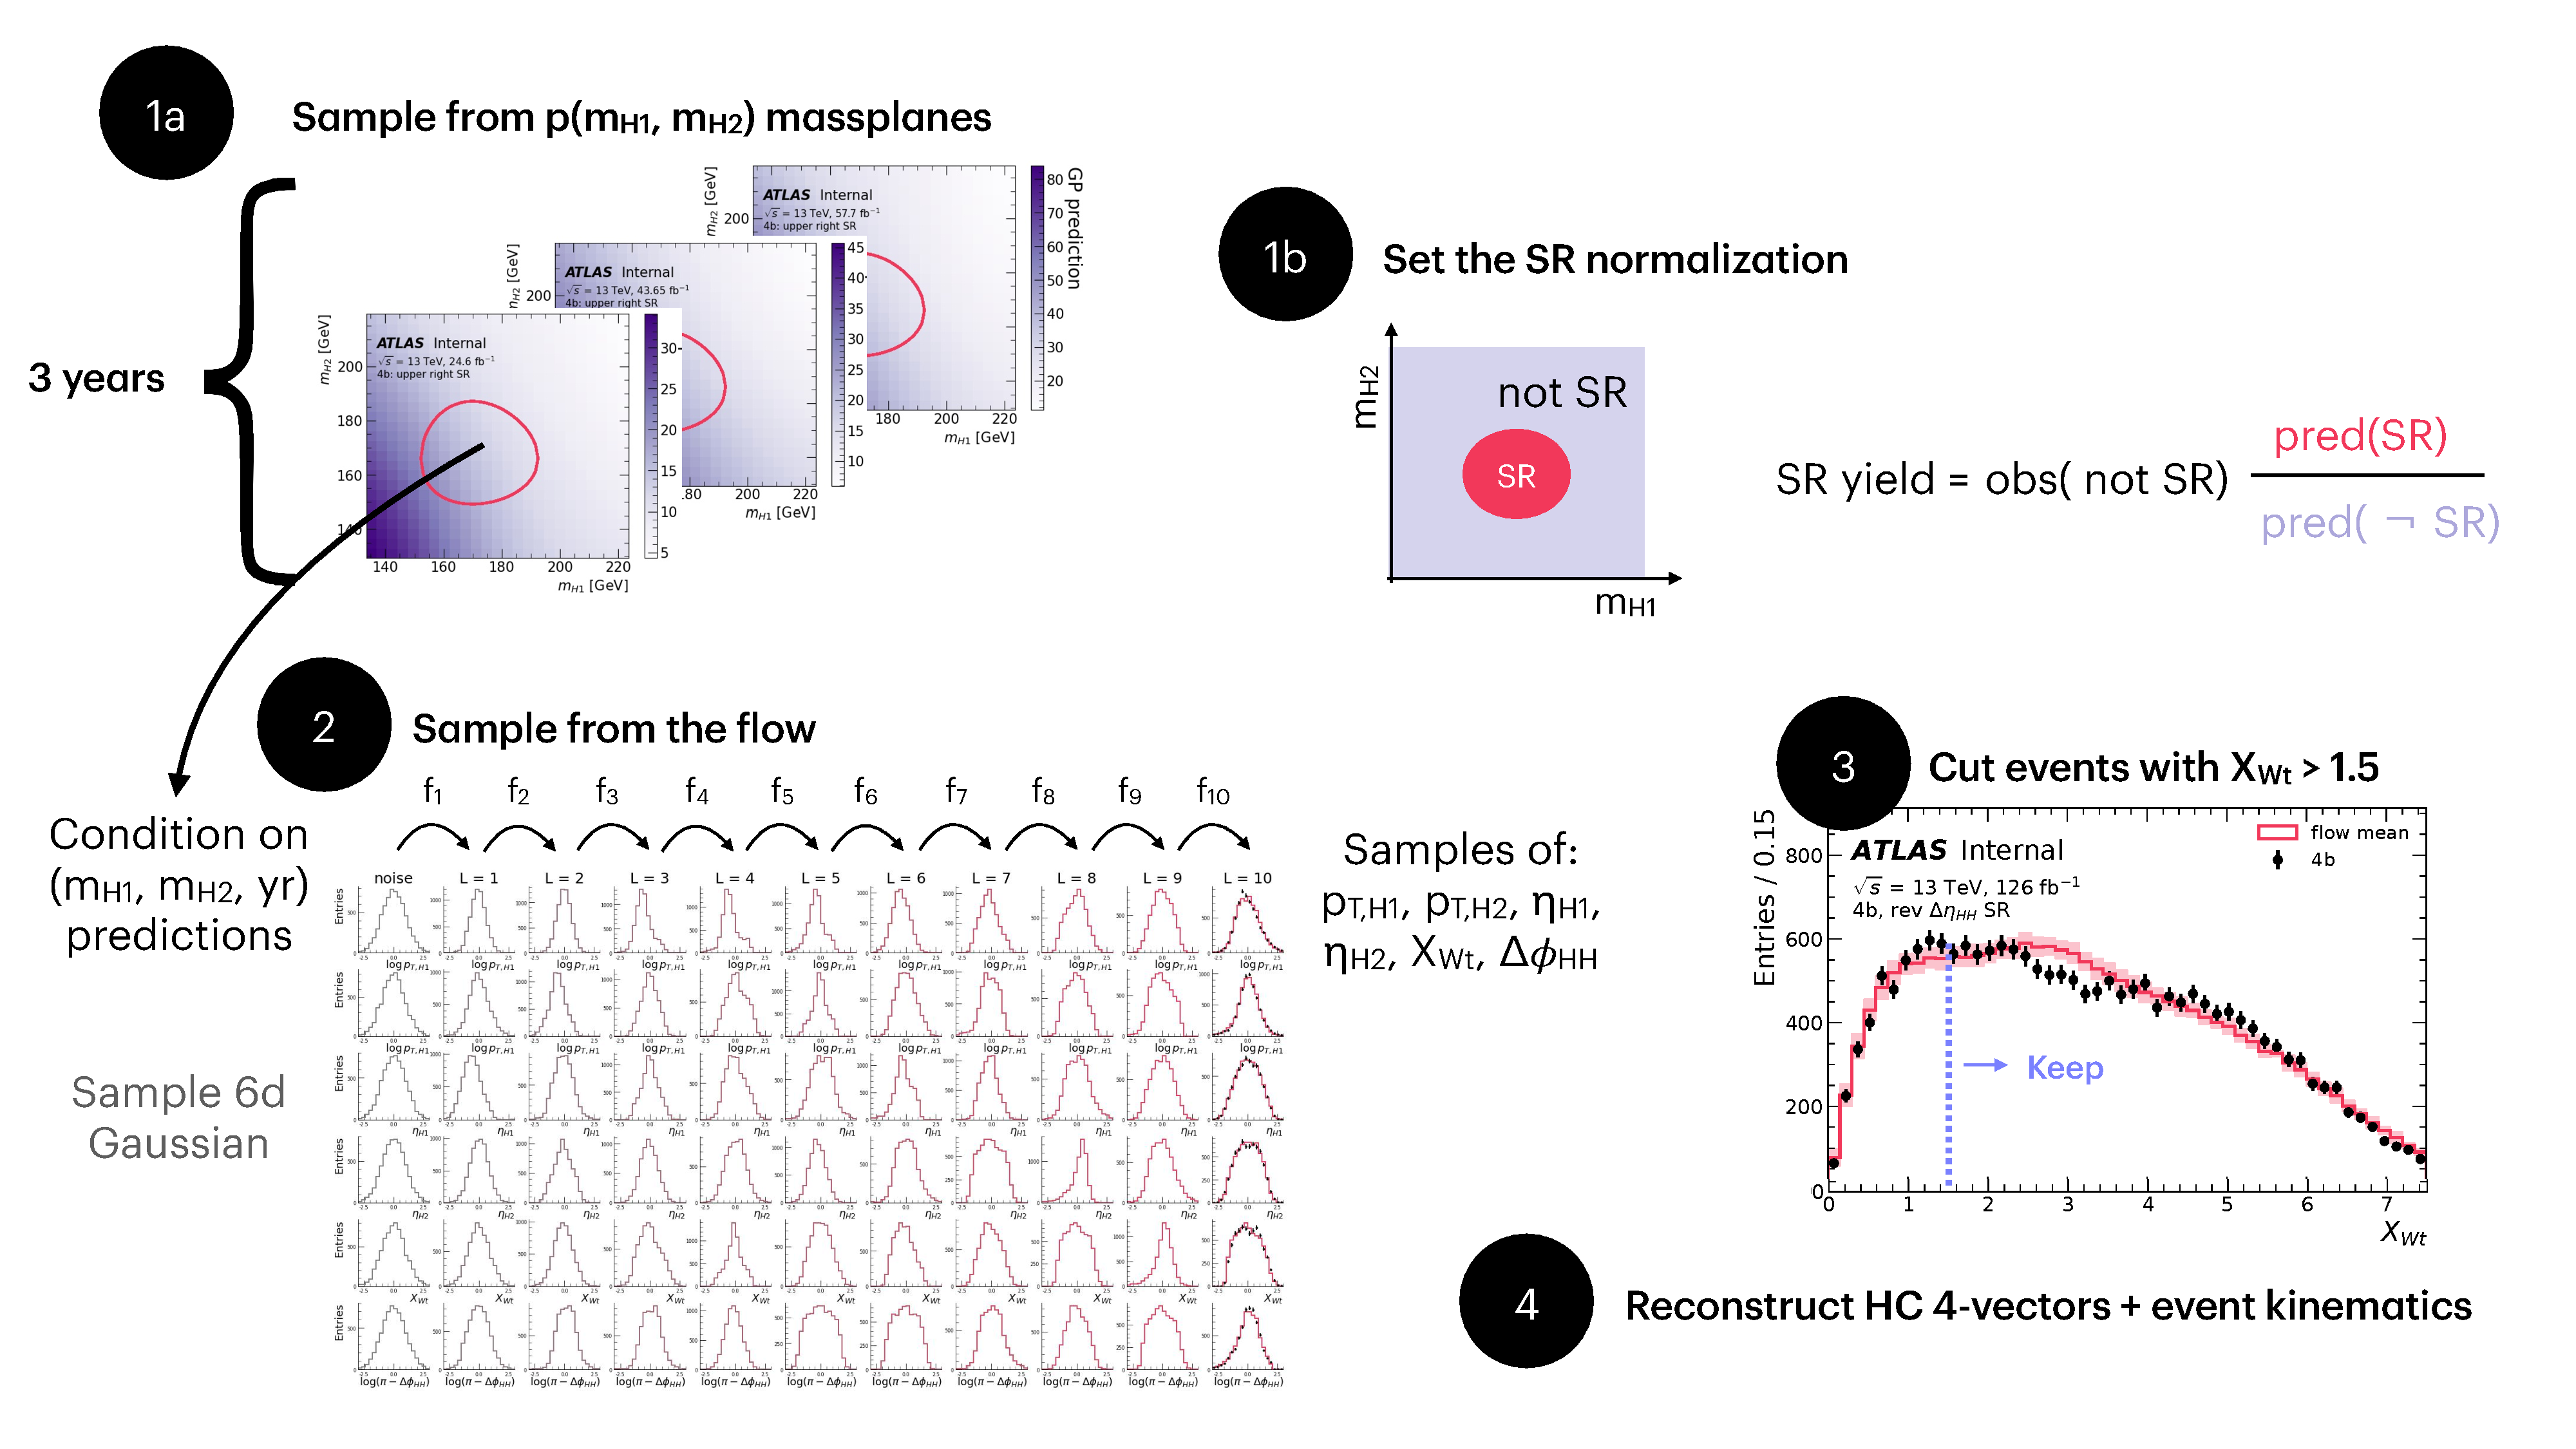
\includegraphics[width=\textwidth]{figures//flows/interp-graphic.pdf} 
    \caption{
    		 Demonstration of the background prediction algorithm for the upper right SR. 
		 }
		 \label{fig:interp-graphic-\valreg}
\end{figure}



